\subsection{Overview}

In this paper we describe the Reachable Polyhedral Marching (RPM) algorithm for enumerating the affine regions of neural networks with rectified linear unit (ReLU) activation.
This algorithm can then be leveraged to compute forward and backward reachable sets of neural networks.
Our algorithm provides a building block for proving safety properties for autonomous systems with learned perception, dynamics, or control components in the loop.  
Specifically, given a set in the input space, RPM computes the set of all corresponding outputs. 
Similarly, given a set of outputs, RPM computes the set of all corresponding inputs under the ReLU network.  
We use these capabilities to compute control invariant sets and regions of attraction (ROAs) for dynamical systems represented as neural networks.
Computing these sets helps roboticists (i) verify whether safety specifications on the robot state are met, (ii) identify states that will converge to some desirable equilibria, and (iii) identify regions in the state space for which a system can be controlled.
Identification of these sets is an important part of the control design process, as directly synthesizing control policies that meet invariance constraints by construction is challenging \cite{blanchini2008set}.
If a constraint is not met, the reachable or invariant sets computed give insight into which states lead to violation of the constraints, informing targeted policy improvements.

% Forward and backward reachable sets are often used in robotics to assess safety. 
% When a robot has a goal set of states to reach and an unsafe set of states to avoid, finding a forward reachable set can determine whether a set of initial states will reach the goal set and avoid the unsafe set. 
% Conversely, finding backward reachable sets of the goal and unsafe sets can determine which initial states will reach the goal and which will lead to the unsafe set. 

% While forward and backward reachable sets are useful to assess safety, the cost of computing these sets scales poorly with the number of time steps into the future or past. 
% For longer time horizons it is often more feasible to search for \textit{invariant sets}. 
% An invariant set is a set of states such that all trajectories starting within the set never leave the set.
% When all trajectories in an invariant set asymptotically converge to an equilibrium, the set is called an invariant \textit{region of attraction} (ROA).



\begin{figure}[!t]
    % \setlength\abovecaptionskip{-0.2\baselineskip}
  % \setlength\belowcaptionskip{-1.5\baselineskip}
  \centering
%   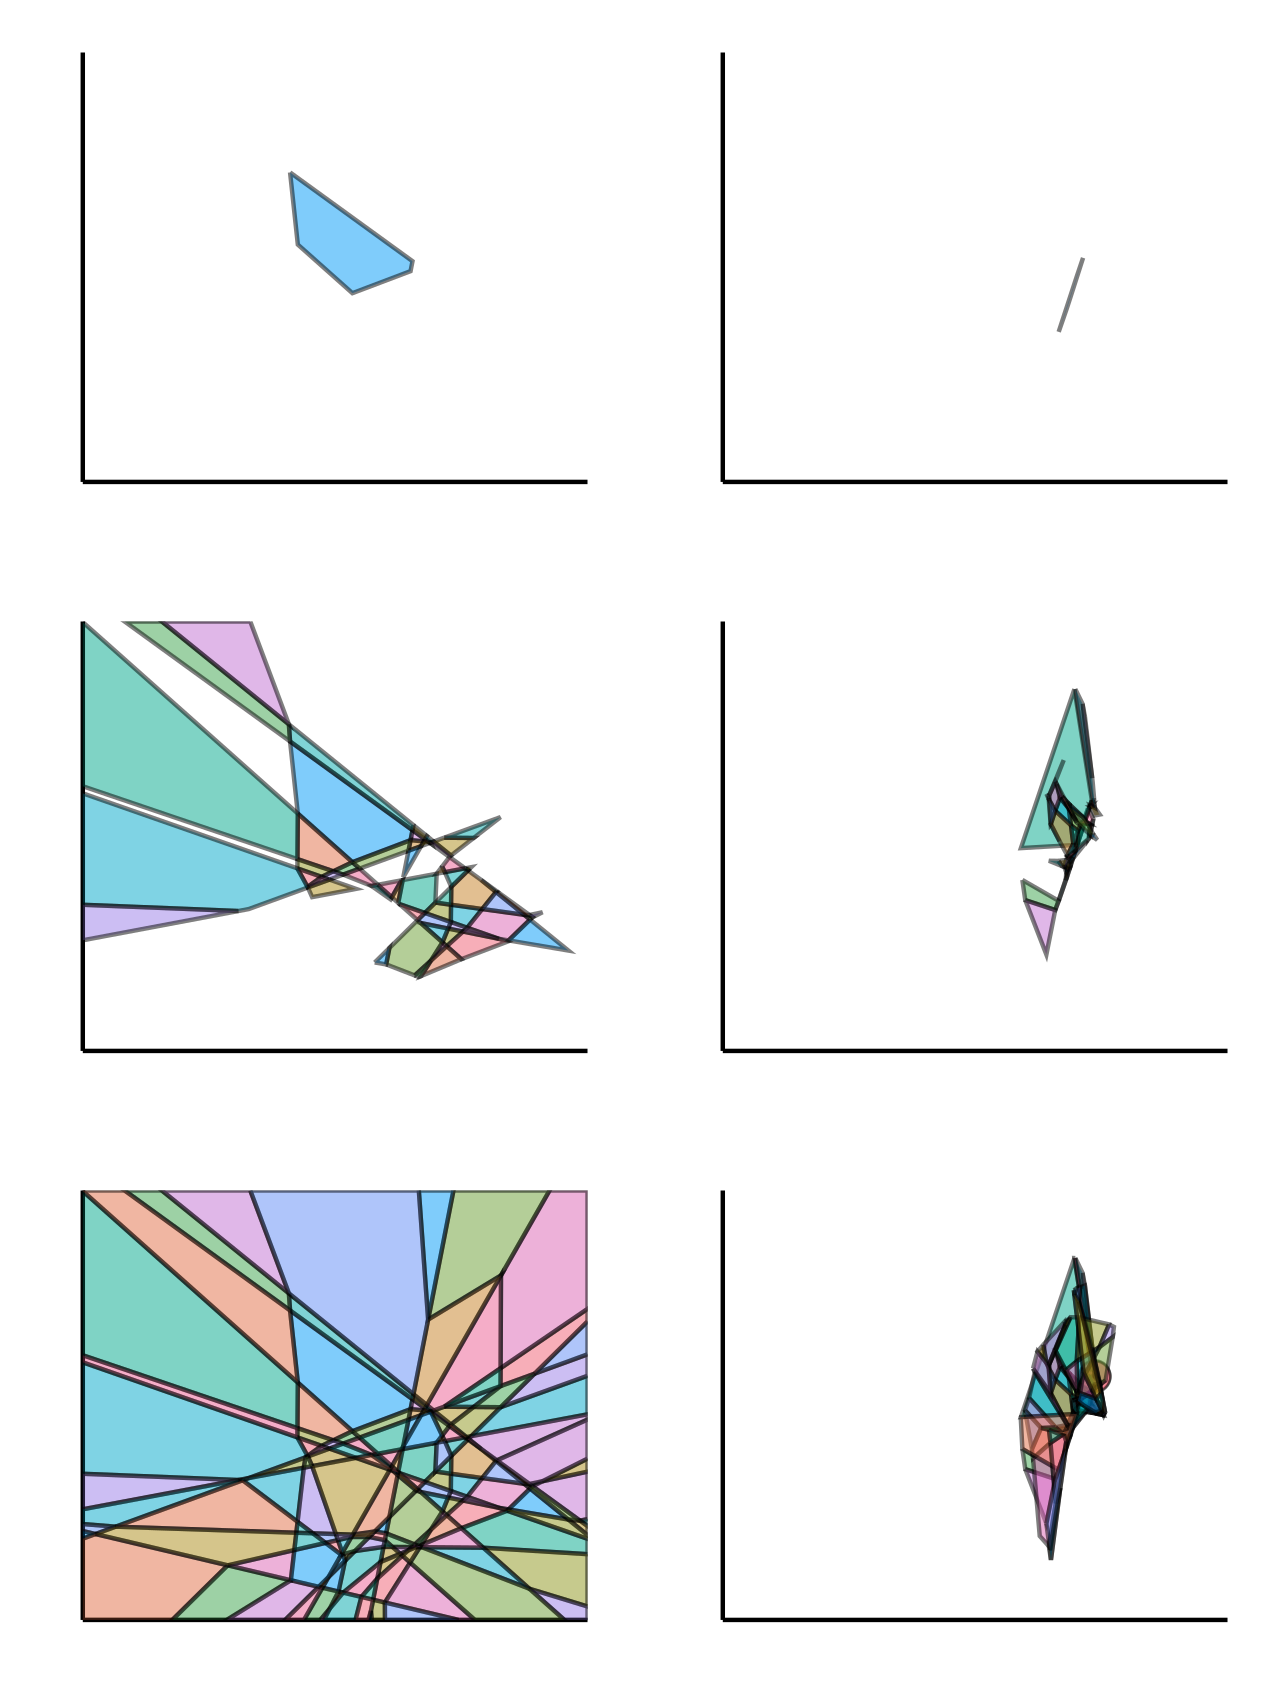
\includegraphics[width=\columnwidth]{figs/figure_1.png}
  % \includesvg[width=\columnwidth]{figs/figure_1.svg}
  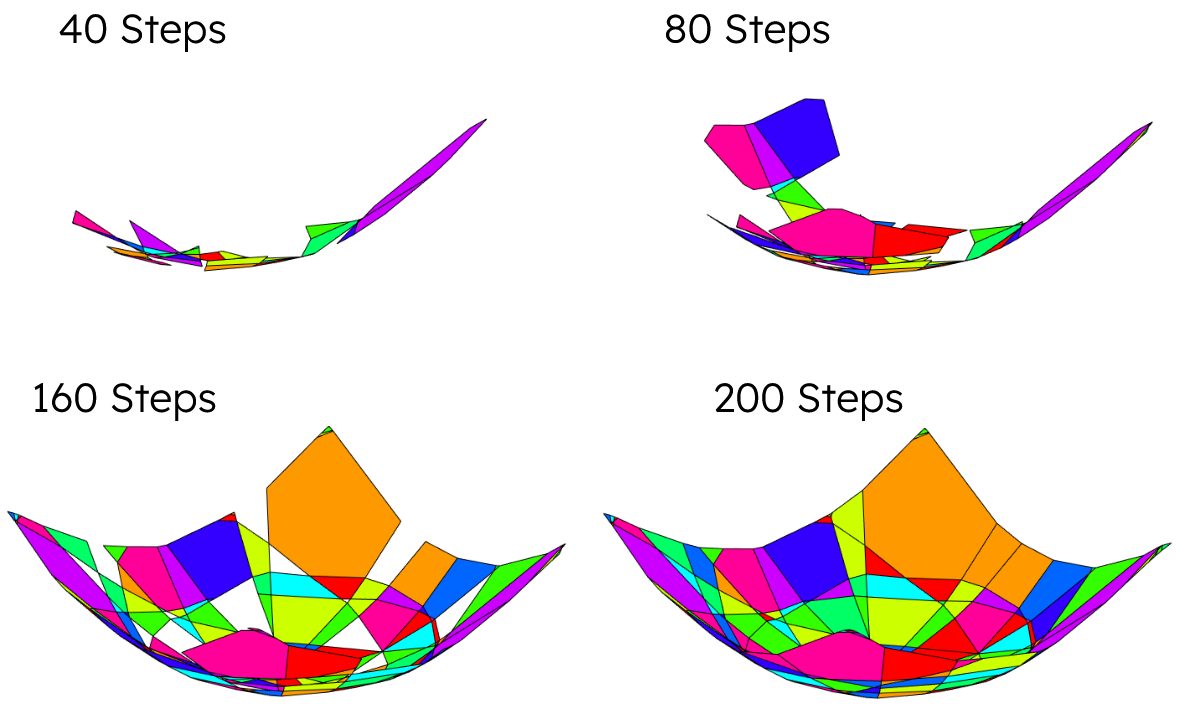
\includegraphics[width=0.85\columnwidth]{figs/figure_1_nobox.png}
  \caption{RPM's incremental enumeration of each affine region in a ReLU network. In this case the ReLU network was trained to approximate a quadratic function. Each new affine region enumerated is connected to a previous region.}
  \label{fig:cell_enum}
\end{figure}

It is well known that ReLU networks implement continuous piecewise-affine (PWA) functions, that is, the input space for a ReLU network can be tessellated into polyhedra, and over each polyhedron the neural network is affine. 
The RPM algorithm explicitly finds this equivalent PWA representation for a given ReLU network. 
Figure \ref{fig:cell_enum} illustrates how RPM incrementally solves for this representation. 
The algorithm incrementally enumerates the polyhedra and affine pieces of the PWA function by solving a series of Linear Programs (LPs), and following analytical edge flipping rules to determine neighboring polyhedra. 
The algorithm starts with an initial polyhedron, then solves for its neighboring polyhedra, then neighbors of neighbors, etc., until the desired input set is tessellated. 
In this way, our method is geometrically similar to fast marching methods in optimal control \cite{HJBFastMarching}, path planning \cite{PlanningFastMarching,FMT}, and graphics \cite{FastMarchingCubes,lei2020analytic}. 

We then use methods for PWA reachability to compute forward and backward reachable sets for each polyhedron and associated affine function. 
Computing forward and backward reachable sets allows us to search for and construct control invariant sets and ROAs without Lyapunov tools.
Finally, we also propose an accelerated backward reachability procedure that leverages the connected enumeration of the RPM algorithm to restrict the number of polyhedra the algorithm searches over.
We show that this accelerated procedure is guaranteed to enumerate the entire backward reachable set in the case that the deep network is a homeomorphism (a continuous bijection with continuous inverse).  
Checking this condition is simple, and represents a novel general procedure for examining the invertibility of neural networks whose hidden layers are not invertible themselves.

% While deep learning holds immense promise for expanding the capabilities, flexibility, and adaptability of robotic systems, currently there exists no practical method for verifying dynamic safety properties (such as stability, persistent feasibility, or forward invariance) of robotic systems with learned components.  Developing such safety verification tools is crucial if robots with learned components are to be used in safety critical applications, such as autonomous cars, aircraft, manufacturing, or search and rescue.

\subsection{Existing Work}
Most existing algorithms that compute exact reachable sets of neural networks iterate through the network layer-by-layer \cite{xiang2017reachable,nnv,yang2020reachability}. 
The layer-by-layer approaches obtain the entire reachable set at once at the end of the computation, rather than revealing the reachable set piece by piece throughout the computation. 
Consequently, if the computation must end early due to memory constraints or a computer fault, no usable result is obtained. 
In contrast, RPM builds the reachable set one polyhedron at a time, leading to a partial, but still potentially useful result if computation is halted before the algorithm runs to completion. 
% Incremental computation is better suited to finding counterexamples to safety properties and terminating early, as well as providing a more memory efficient approach where a region of the reachable set already computed can be saved externally to free up memory for remaining computation. 

\textcolor{black}{The authors of \cite{nnenum} also propose an incremental approach to visiting each affine region in a ReLU network.}
The difference between this tool and our RPM algorithm is that RPM enumerates affine regions of the neural network in a connected walk; each new region that is revealed is connected to a previous region. 
In contrast, the algorithm used in \cite{nnenum} does not have this property; whether a new region is connected to a previous one is unknown by the algorithm.
In Section \ref{Sec:ROA} we show how the connected enumeration property leads to an accelerated algorithm for computing ROAs.
Another way to conceptualize this difference between RPM and \cite{nnenum} is that RPM can also return the graph that describes which affine regions neighbor one another. \textcolor{black}{This feature is enabled by RPM's unique property of removing redundant constraints in the input-space polyhedra, resulting in the minimal description of each affine region.}

% The set of polyhedra and associated affine maps produced by our algorithm is an explicit piecewise-affine (PWA) representation of the ReLU network.  Aside from computing reachable sets, this explicit PWA representation provides useful insights such as the number of affine regions and the rank of each affine map.  Dynamical systems with PWA dynamics, known as hybrid systems, are well studied. Hence, using our method to translate a ReLU network to a PWA function, control design and analysis tools from the hybrid systems literature  \cite{invariant} can be immediately applied to dynamics with ReLU components. 

% A key challenge in verifying the safety of robots with learned components is that robots are dynamical systems, iterating their behavior over time in a feedback loop.  Existing neural network verification methods are inadequate, as they are typically not designed for iterative executions of the network in a feedback loop, are often limited to impractically small networks, and rarely consider backward reachability.  In contrast, our algorithm is designed to quickly determine reachable sets over multiple time steps into the future or the past.  Our algorithm could be used within a planning algorithm to determine, e.g., if a collision is imminent, or to perform offline verification to determine if unsafe states are reachable during execution.

 %Neural networks are increasingly used in both the modeling and control of dynamical systems. Neural networks have shown incredible potential for their usefulness in robotics, however, the realization of this potential to real-world and potentially safety-critical systems is dependent on a user's ability to verify the effectiveness and safety of these learned components. In recent years the field of neural network verification has emerged to address the problem of analyzing properties of neural networks over continuous input sets. For example, such properties may include desired input-output behavior of a learned controller, or whether a region of the state space is reachable for a learned dynamical system given a range of initial conditions.  Approaches to neural network verification can largely be characterized as reachability, optimization, and search approaches \cite{liu2019algorithms}. Reachability approaches are especially useful for analysis of learned dynamical systems. In this paper, we consider the problem of determining exact forward and backward reachable sets of a neural network given specified input and output sets, respectively. To this end we propose a novel reachability approach for the analysis of neural networks. 
 \subsection{Contributions and Organization}
\textcolor{black}{In \cite{VincentSchwagerICRA21RPM}, the RPM algorithm was introduced and demonstrated on multi-step reachability tasks. 
In contrast, the contributions of this paper are
\begin{itemize}
     \item \textcolor{black}{A formal proof of correctness for the RPM algorithm via} a theorem to analytically determine an \textcolor{black}{affine region} from its neighbor by flipping neuron activations in ReLU networks. 
     \item Application of PWA analysis tools to compute control invariant sets and regions of attraction for dynamical systems represented as ReLU networks.
     \item An accelerated exact backward reachability algorithm for ReLU networks \textcolor{black}{that does not require enumerating all affine regions}, leveraging a novel \textcolor{black}{approach} for checking the invertibility of the network.
\end{itemize}}


\textcolor{black}{Through these contributions,} we are able to compute intricate invariant sets that may be non-convex and even disconnected.
In numerical examples, we compute ROAs for a learned van der Pol oscillator, and show this computation enjoys a $15$x speedup because the learned dynamics are homeomorphic. 
We then pair RPM with the MPT3 \cite{MPT3} Matlab toolbox to find an a control invariant set for a learned torque-controlled pendulum. 
Finally, we apply our algorithm to find a set of states stabilized by an image-based airplane runway taxiing system, TaxiNet \cite{verify_gan}. 
The closed-loop system is PWA with ${\sim}250,000$ regions, orders of magnitude larger than PWA systems for which other nonlinear stability analysis approaches have been demonstrated.

The paper is organized as follows.
We give related work in Section \ref{Sec:RelatedWork} and give background and state the problem in Section \ref{Sec:Background}. 
Section \ref{Sec:PWA} describes the RPM algorithm and explains its derivation. 
In Section \ref{Sec:Reachability} we describe how RPM is used to perform forward and backward reachability computations for ReLU networks over multiple time steps. 
In Section \ref{Sec:ROA} we describe how RPM is leveraged to compute control invariant sets and ROAs. 
Finally, Section \ref{Sec:Examples} presents numerical results for computing control invariant sets and ROAs for learned dynamical systems and we offer conclusions in Section \ref{Sec:Conclusions}. 
% \textcolor{black}{
% In the Appendix we provide discussion and a numerical example of using RPM for the neural network verification problem as well as provide a proof for the correctness of the RPM algorithm.}

% Within the reachability approaches, there is a distinction between exact methods and overapproximate methods. Given a set of possible inputs, exact methods determine the image of the input set while overapproximate methods solve for an output set that is guaranteed to be a superset of the image of the input set. Overapproximate methods tend to scale better than exact methods, although sometimes the degree of overapproximation can be prohibitive. 

% Exact reachability approaches included [REF][REF]. The approach taken by these works is to apply layer-by-layer set manipulations to propagate the input set through the network. In contrast, our approach is not a layer-by-layer approach. As such, we expect the computational complexity to scale differently and thus expect there are some problems where our method is advantageous over existing methods.